%---------------------------------------------------------
\begin{frame}{A reproducibility problem, Biology}
\begin{center}
   \alert{$70\%$} of the analyses in Experimental Biology are \alert{not} reproducible
   \vfill
   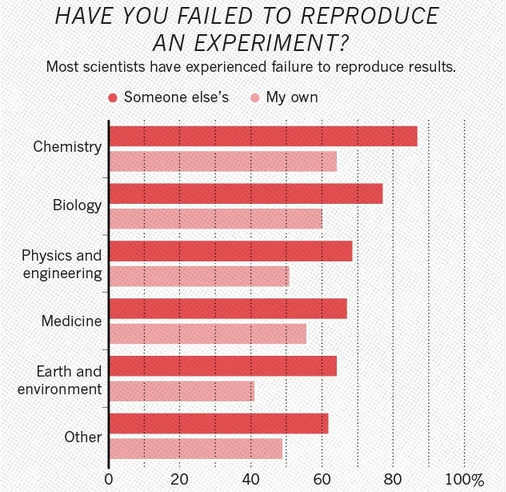
\includegraphics[height=5cm]{01_introduction/images/FAIR_Baker_survey.png}
\end{center}
\tiny{Monya Baker, 1,500 scientists lift the lid on reproducibility, \textit{Nature}, 2016}
\end{frame}
%---------------------------------------------------------
\begin{frame}{A reproducibility problem, Computer Sciences}
    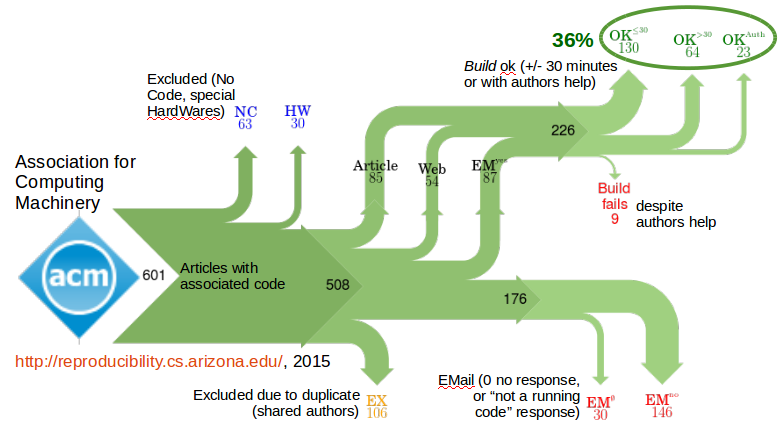
\includegraphics[height=6.4cm]{01_introduction/images/FAIR_acm_study.png}
\end{frame}
%---------------------------------------------------------
\begin{frame}{A reproducibility problem, Bioinformatics}
\begin{columns}
   \column{0.4\textwidth}
   \begin{center}
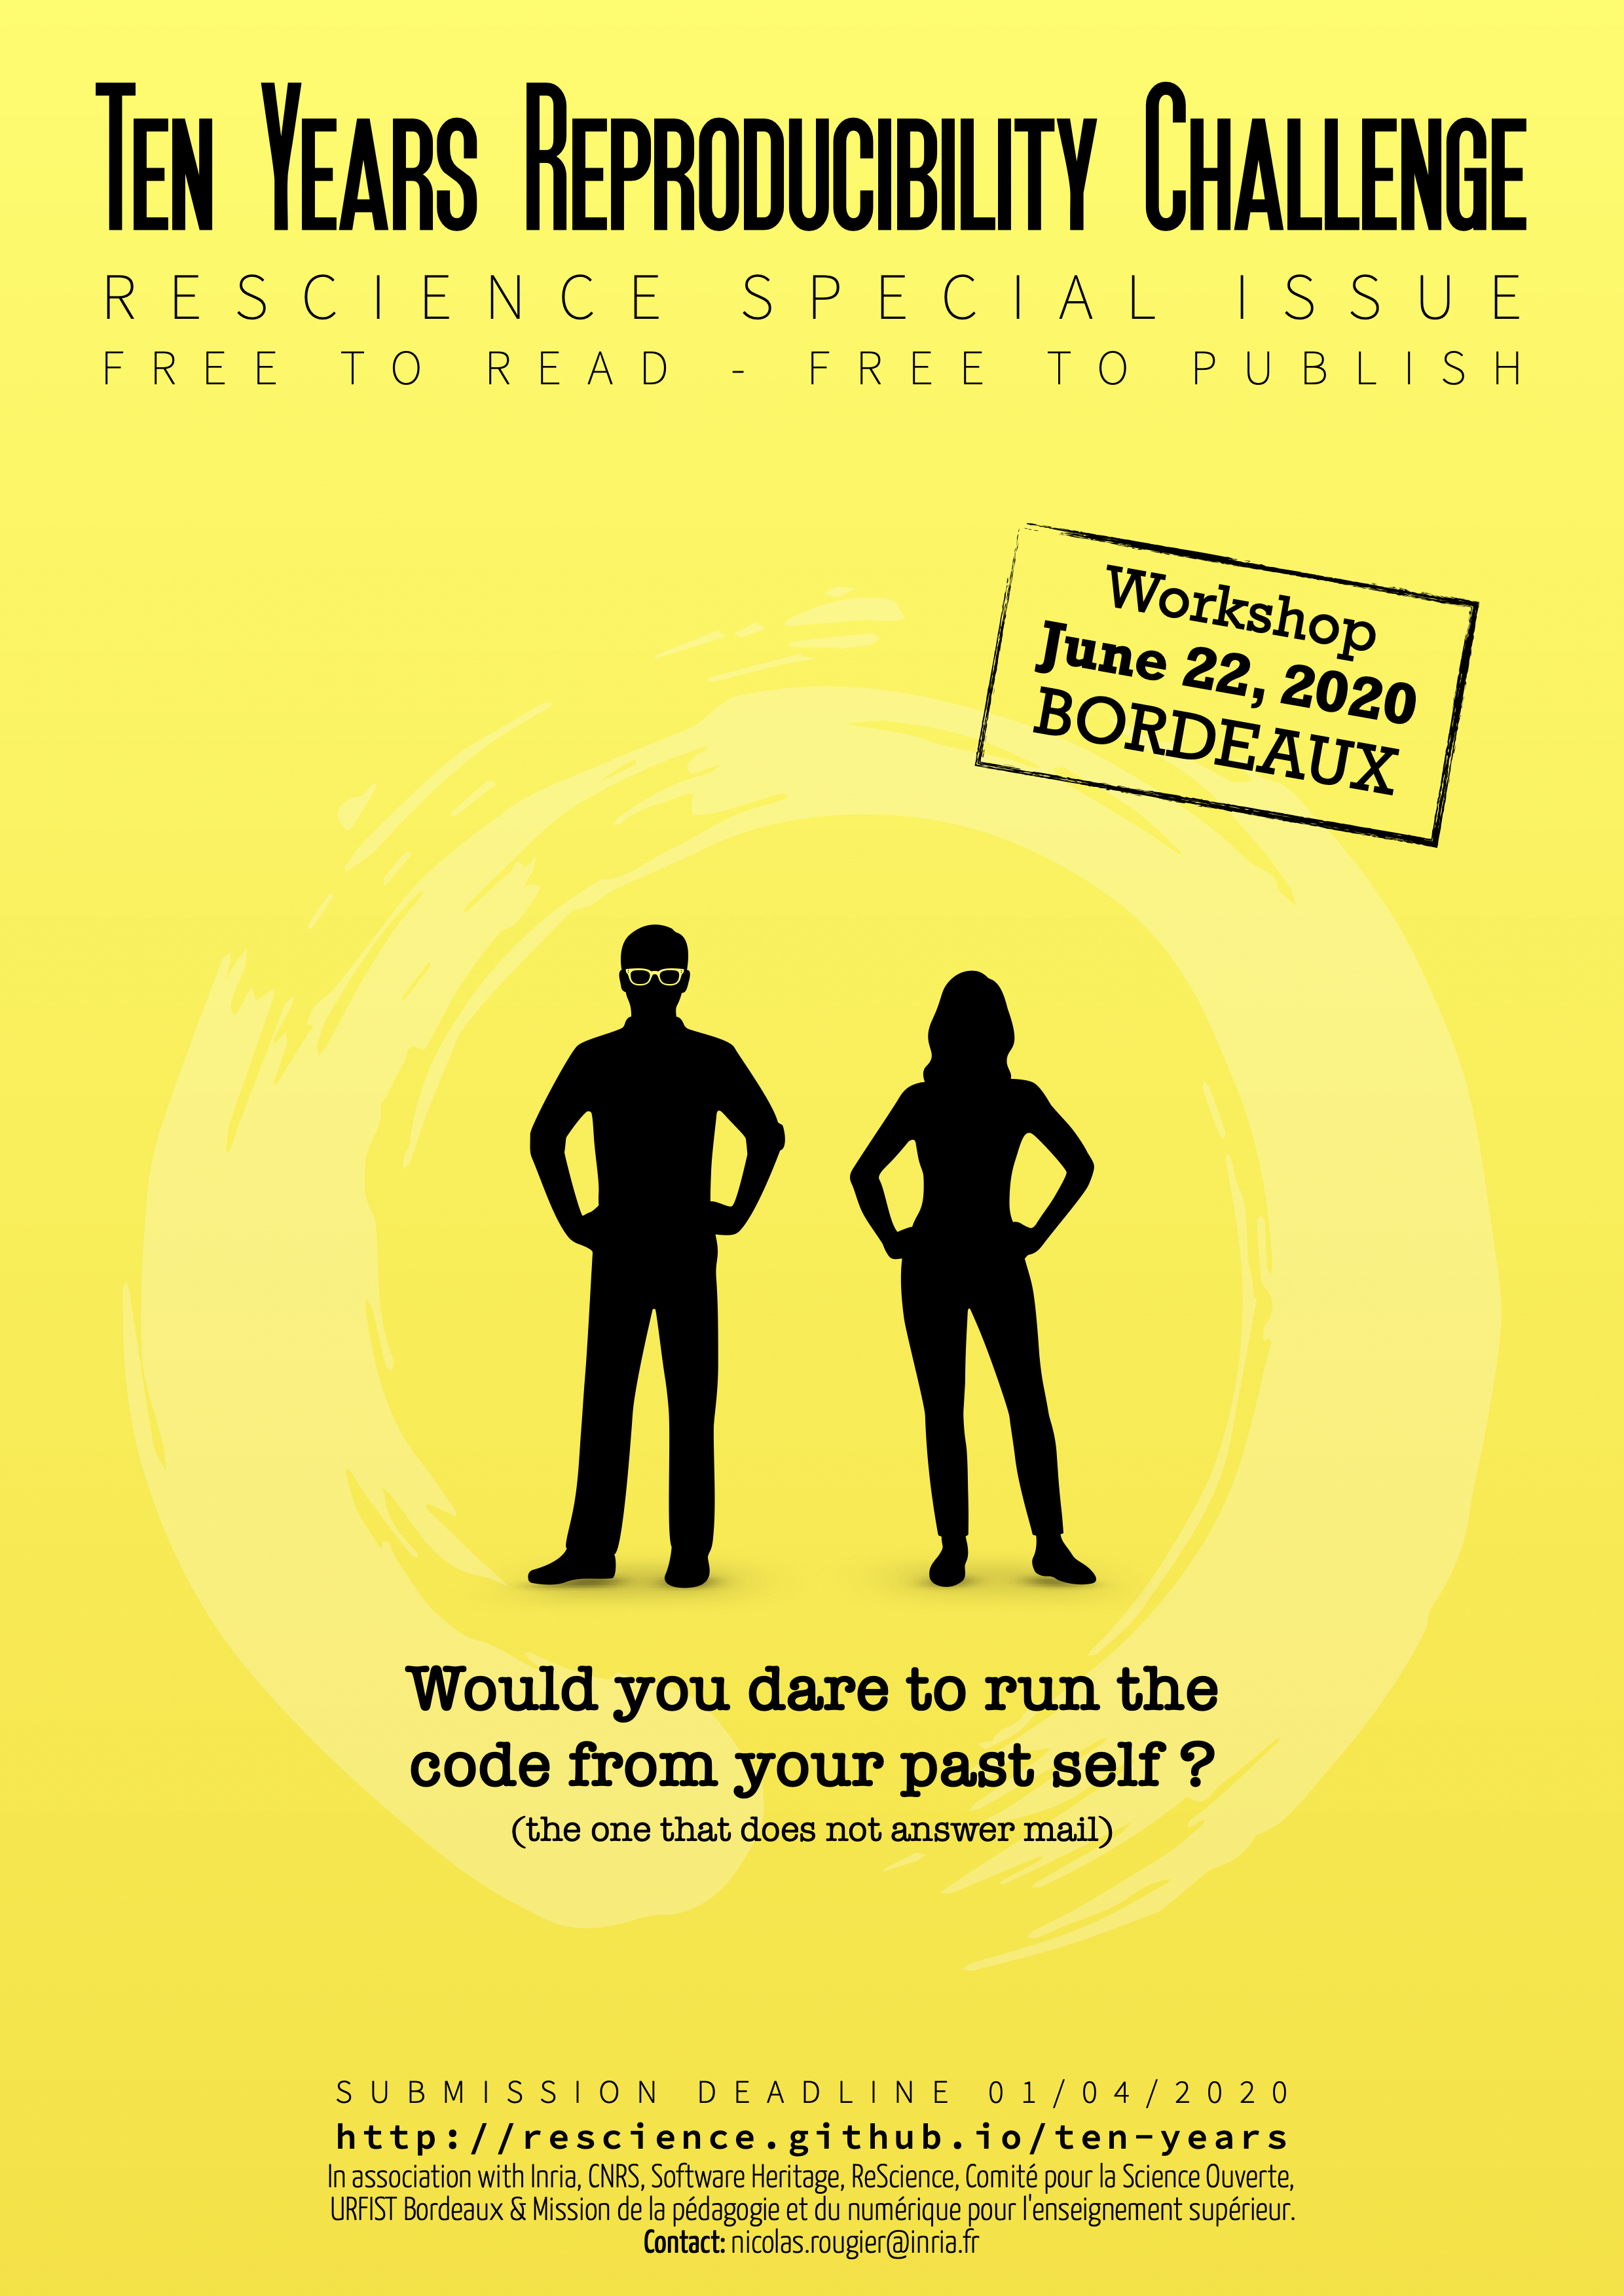
\includegraphics[height=5cm]{01_introduction/images/FAIR_resciences_10-years-challenge.png}
\small{
Ten-Year Reproducibility\\
Challenge, Konrad Hinsen\\
Can your 2009 code still run? \\
special issue of \href{http://rescience.github.io/ten-years}{\textcolor{blue}{\underline{ReScience}}} and \href{https://www.nature.com/articles/d41586-020-02462-7}{\textcolor{blue}{result comments}} in \textit{Nature}
}
   \end{center}
  \column{0.6\textwidth}
Who's never wanted to take over a protocol, a pipeline, or a tool without running into it?
\begin{itemize}
    \item unable to install tools: not compatible OS, not availability of dependencies
    \item tool update $\Rightarrow$ codes unusable: python 2 vs. 3, change of function arguments (R)
    \item inability to reproduce the results of computational analysis: package versions, IDE: stable version of the language different according to the OS (Rstudio)
\end{itemize}
\end{columns}
\end{frame}
%---------------------------------------------------------
\begin{frame}{Reproducibility in science}
\textit{Reproducible research, Repeatability, Replicability, Reproducibility, Replication:} overlapping semantics $\Rightarrow$ a plethora of definitions$!^{a}$\\
\begin{columns}
    \begin{column}{3.5cm}
      \begin{center}
      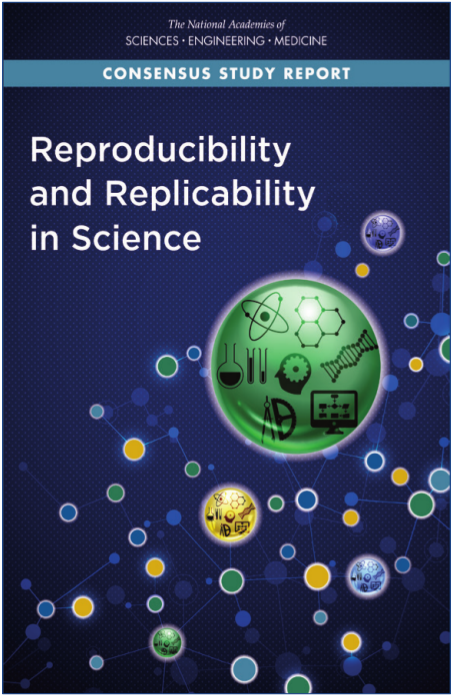
\includegraphics[height=4cm]{01_introduction/images/FAIR_reproducibilityUSA.png}\\
      National Academies of Sciences, Engineering, and Medicine (2019)$.^{b}$
      \end{center}
    \end{column}
    \begin{column}{8.5cm}
      ACM definition (2016):
      \begin{description}
          \item [Repeatability] Same team, same exp. setup
          \item [Replicability] Different team, same exp. setup
          \item [Reproducibility] Different team, different exp. setup
      \end{description}
      \vfill
      Whitaker's matrix of reproducibility (2017)$:^{c}$
      \begin{center}
         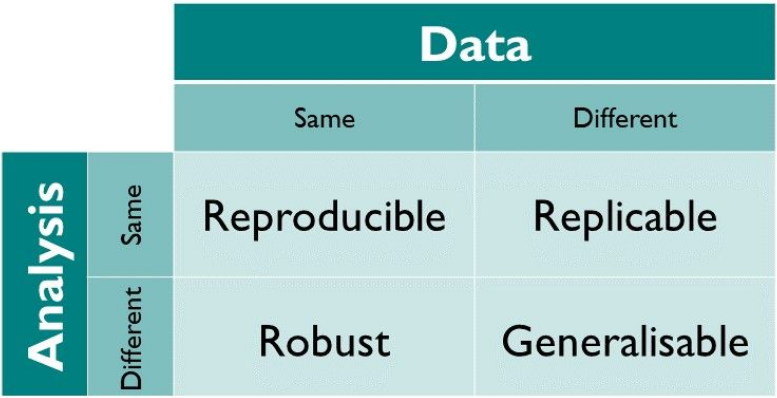
\includegraphics[height=2.5cm]{01_introduction/images/FAIR_Whitaker_matrix_RRRG.png}\\
      \end{center}
    \end{column}
\end{columns}
\tiny{a: \url{https://www.researchgate.net/publication/323118701_Terminologies_for_Reproducible_Research}\\
      b: National Academies of Sciences, Engineering, and Medicine. 2019. Washington DC. The National Academies Press, \url{https://www.nap.edu/read/25303/chapter/1}\\
      c: \url{https://doi.org/10.6084/m9.figshare.5443201.v1}, Slide number 7}
\end{frame}
%---------------------------------------------------------
\begin{frame}{FAIR$\_$bionfo's finding}
Depends on the object of study x \\
\quad \quad \quad what needs to be "memorized" to replay the experience:
\begin{columns}[t]
  \begin{column}{.3\textwidth}\begin{center}
        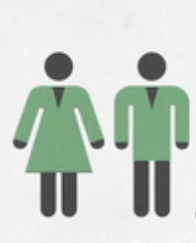
\includegraphics[height=1.2cm]{01_introduction/images/FAIR_Baker_data.png}\\
        \textcolor{blue}{Raw Data}\\FAIR data principles $\&$ Data Management Plans
      \end{center}\end{column}
      \begin{column}{.05\textwidth}\begin{center}
         $\rightarrow$
      \end{center}\end{column}
      \begin{column}{.3\textwidth}\begin{center}
         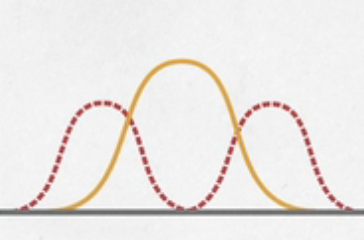
\includegraphics[height=1.2cm]{01_introduction/images/FAIR_Baker_process.png}\\
         \textcolor{blue}{Statistical or bioinformatic analysis}\\Codes - algorithms - workflows
      \end{center}\end{column}
      \begin{column}{.05\textwidth}\begin{center}
         $\rightarrow$
      \end{center}\end{column}
      \begin{column}{0.3\textwidth}\begin{center}
         
\includegraphics[height=1.2cm]{01_introduction/images/FAIR_Baker_results.png}\\
         \textcolor{blue}{Validation}\\Publication: thesis, article, report, etc
        \end{center}\end{column}
  \end{columns}
  \begin{block}{How to gain in reproductibility?}
   Focus on codes, algorithms, workflows used throughout the process
  \end{block}
  \vfill
  \tiny{Monya Baker, 1,500 scientists lift the lid on reproducibility, \textit{Nature}, 2016}
\end{frame}
